\section{Эффекти Кречмана}
\begin{center}
	\begin{tikzpicture}
	
	\node[] at (60:1.5)  {$\theta$};
	\node[] at (35:1)  {$\alpha$};
	\node[] at (12:6.2)  {$\beta$};
	\coordinate (fov) at (2, 1);
	
	\draw[thick,blue, snake=coil,segment aspect=0.15] (fov) -- ++(220:1.5cm);
	\draw[thick,red, snake=coil,segment aspect=0.15] (fov) -- ++(150:3cm);
	\draw[thick,green, snake=coil,segment aspect=0.15] (5,1) -- ++(30:2cm);
	
	\draw[thick] (1,1) arc (180:215:1) ;
	\draw[thick] (0.9,1) arc (180:150:1) ;
	\draw[thick] (5.7,1) arc (0:30:0.6) ;
	\draw[thick,->](8,1) -- (-1,1)  ;
	
	
	\definecolor{color1}{RGB}{252,156,12};
	\definecolor{color2}{RGB}{252,124,12};
	\definecolor{color3}{RGB}{252,104,12};
	\fill[fill=color1,opacity=.7]  (2,0) rectangle (3,2) ;
	\fill[fill=color2,opacity=.7]  (3,0) rectangle (4,2) ;
	\fill[fill=color3,opacity=.7]  (4,0) rectangle (5,2) ;
	\end{tikzpicture}
\end{center}



Рассмотрим падение света на слоистую среду под углом $ 
\theta_1 $ с коэффицентами  диэлектрическими проницаемостями $ \varepsilon_1, \varepsilon_2, \varepsilon_3 $ соответственно. 
На границе каждой среды можно записать закон Снеллиуса.

	$$
	\frac{\sin{\theta_2}}{\sin{\theta_1}} = \frac{n_2}{n_1} =\sqrt{\frac{\varepsilon_{2}}{\varepsilon_1}}	$$
	$$
	\frac{{\sin\theta_3}}{\sin{\theta_2}} = \frac{n_3}{n_2} =\sqrt{\frac{\varepsilon_{3}}{\varepsilon_2}}	
	$$

Наша цель посчитать коэфиценты отражение и прохождения для такой слоистой системы. В это задаче очень полезен метод $ T $-матриц. Обозначим коэффицент отражения через $ r $ , f коэффицент прохождения через $ t $.

Тогда на матричном языке можно задать взаимосвязь между этими величинами. А именно распишем ампплитуды волн слева и справа.

$$\vec{E}=\vec{E}(x) e^{i(\omega t-\beta z)}$$

$$E(x)=\left\{\begin{array}{c}
E_{1} e^{i k_{1} x}+E_{1}^{\prime} e^{-i k_{1} x}, x<0 \\
E_{2} e^{i k_{2 x} x}+E_{2}^{\prime} e^{-i k_{2} x_{2} x}, 0<x<d \\
E_{3} e^{i k_{3}(x-d)}+E_{3}^{\prime} e^{-i k_{3}(x-d)}, x>d
\end{array}\right.$$

$$P_{2}=\left(\begin{array}{cc}
e^{i k_{2 x} d} & 0 \\
0 & e^{-i k_{2 x} d}
\end{array}\right)$$



$$
S_{21} = 
\frac{1}{2 Z_2}\begin{pmatrix}
	Z_2+Z_1 & Z_2 -Z_1 \\
	Z_2-Z_1 & Z_2+Z_1
\end{pmatrix}
$$


$$
S_{32} = 
\frac{1}{2 Z_3}\begin{pmatrix}
Z_3+Z_2 & Z_3 -Z_2 \\
Z_3-Z_2 & Z_3+Z_2
\end{pmatrix}
$$

Где $Z_i = \frac{k_{zi}}{k_0}$ для $ s $ - поляризации и $Z_i = \frac{k_{zi}}{\varepsilon_i k_0}$ для $ p $ - поляризации 

$$
 k_{zi} = \sqrt{k_0^2 \epsilon_i - k_x^2)}
$$

$$
 k_{x} = k_0 \sin{ \theta}
$$


$
S_{32} P_2 S_{21} \begin{pmatrix}
	1\\
	r 
\end{pmatrix} = 
\begin{pmatrix}
t\\
0 
\end{pmatrix}
$


\begin{figure}[h!]
	\centering
	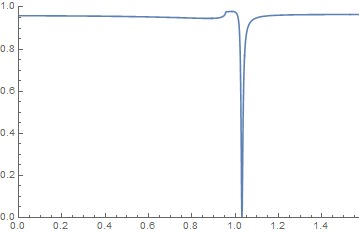
\includegraphics[width=0.7\linewidth]{kretchmann}
	\caption[Эффект Кречмана]{}
	\label{fig:kretchmann}
\end{figure}





